\documentclass[border=14pt]{standalone}
\usepackage[utf8]{inputenc}
\usepackage[T1]{fontenc}
\usepackage{amsmath,amssymb}
\usepackage{tikz}
\usetikzlibrary{arrows.meta,positioning,fit,calc,backgrounds}

\definecolor{CoreNavy}{RGB}{72,92,120}
\definecolor{MutedRust}{RGB}{174,112,96}
\definecolor{MutedTeal}{RGB}{92,146,142}
\definecolor{PaleBlue}{RGB}{235,241,247}
\definecolor{PaleTeal}{RGB}{232,244,242}
\definecolor{PalePeach}{RGB}{248,238,231}
\definecolor{SoftGray}{RGB}{244,245,246}
\definecolor{MidGray}{RGB}{153,160,168}
\definecolor{Ink}{RGB}{40,45,52}

\tikzset{
  >={Stealth[length=2.2mm,width=1.5mm]},
  card/.style={
    draw=CoreNavy,
    fill=white,
    line width=0.9pt,
    rounded corners=2.5mm,
    align=left,
    inner xsep=3.5mm,
    inner ysep=3.0mm,
    text width=62mm,
    font=\sffamily\footnotesize,
    text=Ink
  },
  titlebanner/.style={
    draw=CoreNavy,
    fill=PaleBlue,
    line width=1.0pt,
    rounded corners=2.5mm,
    align=center,
    inner xsep=4mm,
    inner ysep=3mm,
    text width=217mm,
    font=\sffamily\small,
    text=Ink
  },
  flow/.style={->,draw=CoreNavy,line width=1.1pt},
  warnflow/.style={->,draw=MutedRust,line width=1.1pt}
}

\begin{document}
\hbadness=10000\relax
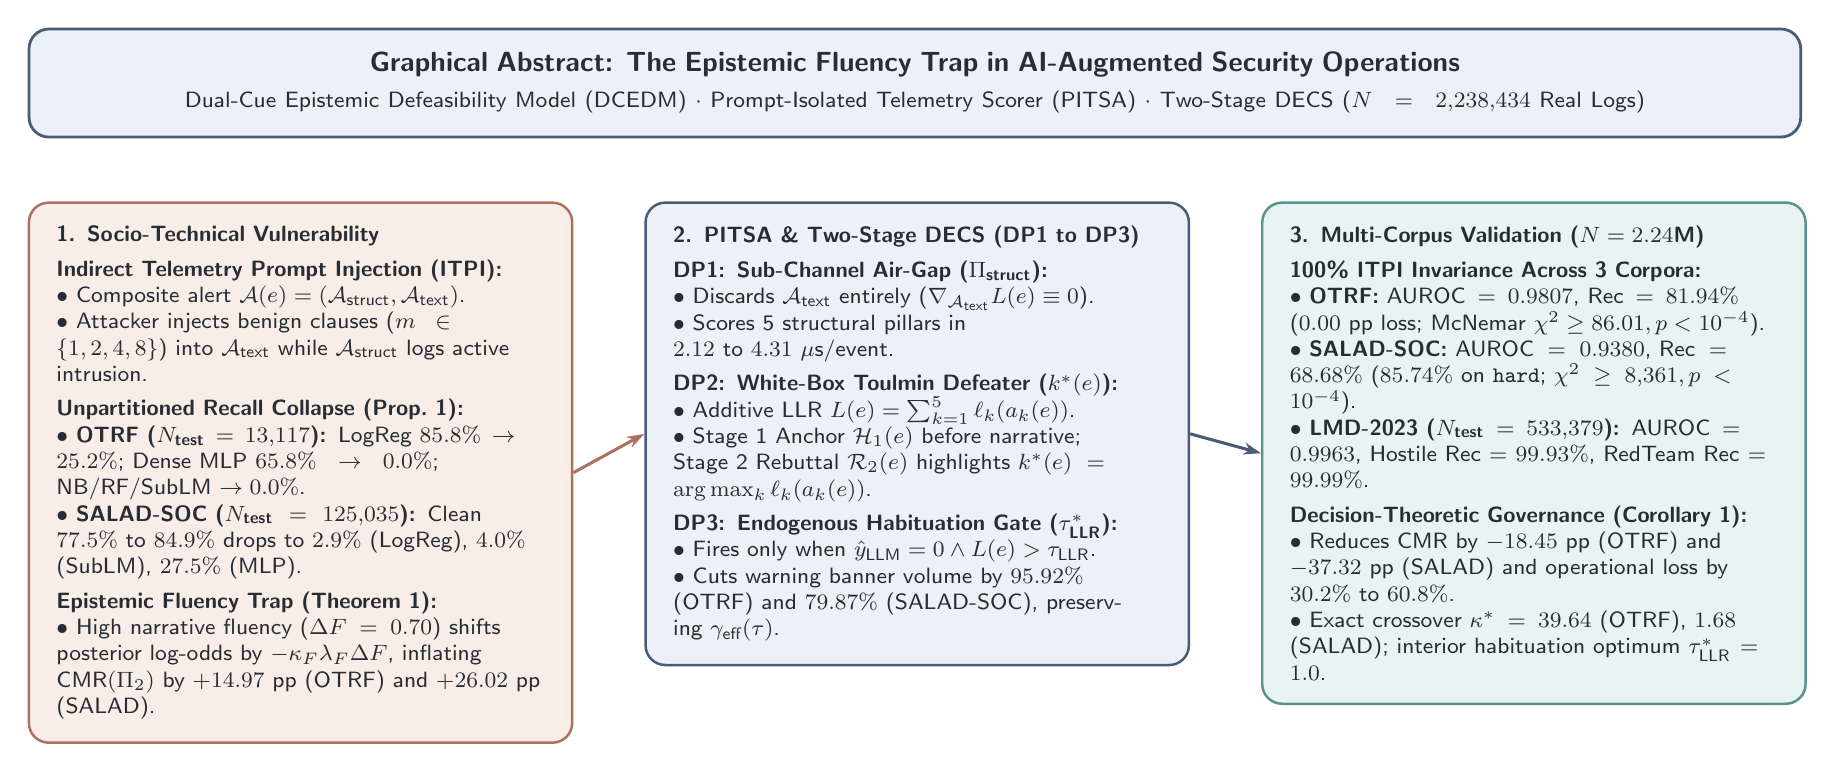
\begin{tikzpicture}[node distance=8mm and 9mm]

  \node[titlebanner] (header) {
    {\normalsize\bfseries Graphical Abstract: The Epistemic Fluency Trap in AI-Augmented Security Operations}\\[2pt]
    \footnotesize Dual-Cue Epistemic Defeasibility Model (DCEDM) $\cdot$ Prompt-Isolated Telemetry Scorer (PITSA) $\cdot$ Two-Stage DECS ($N = 2{,}238{,}434$ Real Logs)
  };

  \node[card, fill=PalePeach, draw=MutedRust, below left=8mm and 0mm of header.south west, anchor=north west] (col1) {
    {\bfseries 1. Socio-Technical Vulnerability}\\[3pt]
    \textbf{Indirect Telemetry Prompt Injection (ITPI):}\\
    $\bullet$ Composite alert $\mathcal{A}(e) = (\mathcal{A}_{\text{struct}}, \mathcal{A}_{\text{text}})$.\\
    $\bullet$ Attacker injects benign clauses ($m \in \{1,2,4,8\}$) into $\mathcal{A}_{\text{text}}$ while $\mathcal{A}_{\text{struct}}$ logs active intrusion.\\[3pt]
    \textbf{Unpartitioned Recall Collapse (Prop.\ 1):}\\
    $\bullet$ \textbf{OTRF ($N_{\text{test}}=13{,}117$):} LogReg $85.8\% \to 25.2\%$; Dense MLP $65.8\% \to 0.0\%$; NB/RF/SubLM $\to 0.0\%$.\\
    $\bullet$ \textbf{SALAD-SOC ($N_{\text{test}}=125{,}035$):} Clean $77.5\%\text{ to }84.9\%$ drops to $2.9\%$ (LogReg), $4.0\%$ (SubLM), $27.5\%$ (MLP).\\[3pt]
    \textbf{Epistemic Fluency Trap (Theorem 1):}\\
    $\bullet$ High narrative fluency ($\Delta F = 0.70$) shifts posterior log-odds by $-\kappa_F \lambda_F \Delta F$, inflating $\text{CMR}(\Pi_2)$ by $+14.97\text{ pp}$ (OTRF) and $+26.02\text{ pp}$ (SALAD).
  };

  \node[card, fill=PaleBlue, right=9mm of col1.north east, anchor=north west] (col2) {
    {\bfseries 2. PITSA \& Two-Stage DECS (DP1 to DP3)}\\[3pt]
    \textbf{DP1: Sub-Channel Air-Gap ($\Pi_{\text{struct}}$):}\\
    $\bullet$ Discards $\mathcal{A}_{\text{text}}$ entirely ($\nabla_{\mathcal{A}_{\text{text}}} L(e) \equiv 0$).\\
    $\bullet$ Scores 5 structural pillars in $2.12\text{ to }4.31\text{ }\mu\text{s/event}$.\\[3pt]
    \textbf{DP2: White-Box Toulmin Defeater ($k^*(e)$):}\\
    $\bullet$ Additive LLR $L(e) = \sum_{k=1}^5 \ell_k(a_k(e))$.\\
    $\bullet$ Stage 1 Anchor $\mathcal{H}_1(e)$ before narrative; Stage 2 Rebuttal $\mathcal{R}_2(e)$ highlights $k^*(e) = \arg\max_k \ell_k(a_k(e))$.\\[3pt]
    \textbf{DP3: Endogenous Habituation Gate ($\tau^*_{\text{LLR}}$):}\\
    $\bullet$ Fires only when $\hat{y}_{\text{LLM}}=0 \wedge L(e) > \tau_{\text{LLR}}$.\\
    $\bullet$ Cuts warning banner volume by $95.92\%$ (OTRF) and $79.87\%$ (SALAD-SOC), preserving $\gamma_{\text{eff}}(\tau)$.
  };

  \node[card, fill=PaleTeal, draw=MutedTeal, right=9mm of col2.north east, anchor=north west] (col3) {
    {\bfseries 3. Multi-Corpus Validation ($N=2.24\text{M}$)}\\[3pt]
    \textbf{100\% ITPI Invariance Across 3 Corpora:}\\
    $\bullet$ \textbf{OTRF:} $\text{AUROC}=0.9807$, $\text{Rec}=81.94\%$ ($0.00\text{ pp}$ loss; McNemar $\chi^2 \ge 86.01, p<10^{-4}$).\\
    $\bullet$ \textbf{SALAD-SOC:} $\text{AUROC}=0.9380$, $\text{Rec}=68.68\%$ ($85.74\%$ on \texttt{hard}; $\chi^2 \ge 8{,}361, p<10^{-4}$).\\
    $\bullet$ \textbf{LMD-2023 ($N_{\text{test}}=533{,}379$):} $\text{AUROC}=0.9963$, Hostile $\text{Rec}=99.93\%$, RedTeam $\text{Rec}=99.99\%$.\\[3pt]
    \textbf{Decision-Theoretic Governance (Corollary 1):}\\
    $\bullet$ Reduces CMR by $-18.45\text{ pp}$ (OTRF) and $-37.32\text{ pp}$ (SALAD) and operational loss by $30.2\%\text{ to }60.8\%$.\\
    $\bullet$ Exact crossover $\kappa^* = 39.64$ (OTRF), $1.68$ (SALAD); interior habituation optimum $\tau^*_{\text{LLR}}=1.0$.
  };

  \draw[warnflow] (col1.east) -- (col2.west);
  \draw[flow] (col2.east) -- (col3.west);

\end{tikzpicture}
\end{document}
